\clearpage
\section*{Problem 4}
\markboth{Problem 4}{Problem 4: Part 1}
\addcontentsline{toc}{section}{Problem 4}

\textbf{Problem Statement:} Consider the equation
$$f(x) = 0,$$
where
$$f(x) = x - \frac{1}{2}\left(\cos(x/2) - \left|x - \frac{1}{2}\right|\right).$$

Do the following.

\subsection*{Part 1}
\addcontentsline{toc}{subsection}{Problem 4.1}

Rewrite the equation as a fixed point problem for a function $T(x)$ related to $f(x)$. Prove that $T(x)$ (i) maps the interval $[0.45, 0.55]$ into itself, and (ii) $T(x)$ is contractive on this interval. Based on the theorems in the books and notes, make conclusions about existence and uniqueness of a solution to $f(x) = 0$.

\noindent\rule{\textwidth}{0.4pt}

\vspace{1em}

\textbf{Solution:}

For determining a suitable fixed point function \( T(x) \), we start with the given equation:
\[f(x) = 0 \implies x = \frac{1}{2}\left(\cos(x/2) - \left|x - \frac{1}{2}\right|\right).\]
Thus, we can define the fixed point function as:
\[
T(x) = \frac{1}{2}\left(\cos(x/2) - \left|x - \frac{1}{2}\right|\right).
\]

To get an idea of the behaviours of functions $f(x)$ and $T(x)$, I plotted both in desmos, as shown in \Cref{fig:p04-fx-plot} and \Cref{fig:p04-Tx-plot}. 

In \Cref{fig:p04-Tx-plot}, I can see that $T(x)$ appears to map the interval $[0.45, 0.55]$ into itself. As for locating the fixed point(s), I can see that $T(x)$ intersects the line $y=x$ at a single point in this interval, suggesting a unique fixed point.
The plot of $f(x)$ in \Cref{fig:p04-fx-plot} suggests the same fixed point which corresponds to the root of the equation \(f(x) = 0\).

\begin{figure}[H]
	\centering
	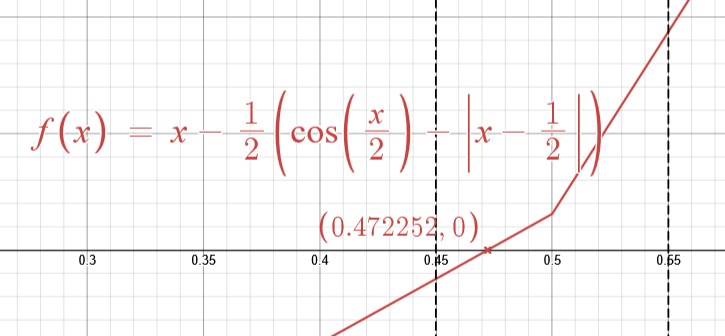
\includegraphics[width=0.7\textwidth]{figures/p04-fx-plot-desmos.png}
	\caption{Plot of $f(x)$ over the relevant interval.}
	\label{fig:p04-fx-plot}
\end{figure}

\begin{figure}[H]
	\centering
	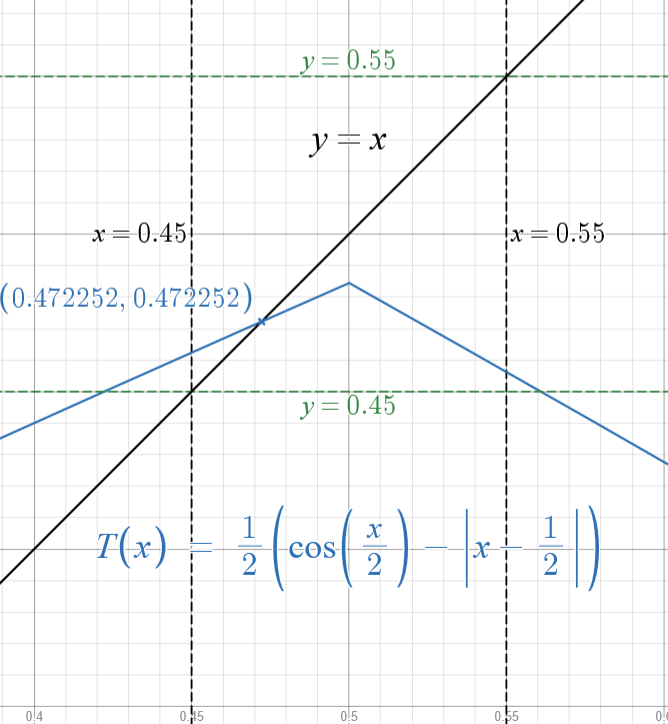
\includegraphics[width=0.7\textwidth]{figures/p04-Tx-plot-desmos.png}
	\caption{Plot of $T(x)$ showing its behavior and mapping in $[0.45, 0.55]$.}
	\label{fig:p04-Tx-plot}
\end{figure}

\vspace{2em}
\noindent\rule{\textwidth}{0.4pt}
